
表达式模板是一种元编程技术,支持在编译时对计算进行惰性计算。这有助于避免在运行时发生低效操作,但这并不是免费的,因为表达式模板需要更多的代码,并且阅读或理解起来可能很麻烦,其经常用于线性代数库的实现。

了解表达式模板之前,先了解它们可以解决什么问题。假设想要对矩阵进行一些操作,实现了基本的操作,加法、减法和乘法(两个矩阵或一个标量和一个矩阵)。可以有以下表达式:

\begin{lstlisting}[style=styleCXX]
auto r1 = m1 + m2;
auto r2 = m1 + m2 + m3;
auto r3 = m1 * m2 + m3 * m4;
auto r4 = m1 + 5 * m2;
\end{lstlisting}

m1, m2, m3和m4是矩阵;类似地,r1, r2, r3和r4是由右边的操作得到的矩阵。第一个操作没有任何问题:m1和m2相加,结果赋值给r1。第二个操作是不同的,因为有三个矩阵相加。所以首先操作m1和m2,并创建一个临时对象,然后将其添加到m3,并将结果分配给r2。

对于第三个操作,有两个临时值:一个是m1和m2相乘的结果,一个是m3和m4相乘的结果;然后这两个相加结果被赋值给r3。最后一个操作类似于第二个操作,所以一个临时对象是由标量5和矩阵m2相乘产生的,然后将这个临时对象添加到m1,并将结果分配给r4。

操作越复杂,生成的临时项就越多。当对象很大时,这会影响性能。表达式模板通过将计算建模为编译时表达式来帮助避免这种情况。整个数学表达式(如m1 + 5 * m2)在计算赋值时变成一个单独的表达式模板,不需要任何临时对象。

为了演示,我们将使用vector而不是矩阵构建一些示例,因为vector是更简单的数据结构,而且练习的重点不是数据的表示,而是表达式模板的创建。下面的代码中,可以看到一个vector类的最小实现,提供了几个操作:

\begin{itemize}
\item
从初始化列表或表示大小的值构造实例(不初始化值)

\item
检索向vector的元素数

\item
使用下标操作符([])访问元素
\end{itemize}

代码如下所示:

\begin{lstlisting}[style=styleCXX]
template<typename T>
struct vector
{
	vector(std::size_t const n) : data_(n) {}
	
	vector(std::initializer_list<T>&& l) : data_(l) {}
	
	std::size_t size() const noexcept
	{
		return data_.size();
	}

	T const & operator[](const std::size_t i) const
	{
		return data_[i];
	}

	T& operator[](const std::size_t i)
	{
		return data_[i];
	}

private:
	std::vector<T> data_;
};
\end{lstlisting}

这看起来非常类似于std::vector标准容器,其在内部会使用这个容器来保存数据,但这与我们要解决的问题无关。这里,使用的是vector,而不是矩阵,因为用几行代码来表示它更容易。有了这个类,就可以定义必要的操作:两个向量之间,以及标量与向量之间的加法和乘法:

\begin{lstlisting}[style=styleCXX]
template<typename T, typename U>
auto operator+ (vector<T> const & a, vector<U> const & b)
{
	using result_type = decltype(std::declval<T>() +
	std::declval<U>());
	vector<result_type> result(a.size());
	for (std::size_t i = 0; i < a.size(); ++i)
	{
		result[i] = a[i] + b[i];
	}
	return result;
}

template<typename T, typename U>
auto operator* (vector<T> const & a, vector<U> const & b)
{
	using result_type = decltype(std::declval<T>() +
	std::declval<U>());
	vector<result_type> result(a.size());
	for (std::size_t i = 0; i < a.size(); ++i)
	{
		result[i] = a[i] * b[i];
	}
	return result;
}

template<typename T, typename S>
auto operator* (S const& s, vector<T> const& v)
{
	using result_type = decltype(std::declval<T>() +
	std::declval<S>());
	vector<result_type> result(v.size());
	for (std::size_t i = 0; i < v.size(); ++i)
	{
		result[i] = s * v[i];
	}
	return result;
}
\end{lstlisting}

这些实现相对简单,在这一点上不应该构成理解问题。+和*运算符都取两个可能类型不同的vector,例如vector<int>和vector<double>,并返回一个包含结果类型元素的向量,是由使用std::declval将模板类型T和U的两个值相加的结果决定的。对于标量和向量相乘,也可以使用类似的实现。有了这些操作符,可以编写如下代码:

\begin{lstlisting}[style=styleCXX]
vector<int> v1{ 1,2,3 };
vector<int> v2{ 4,5,6 };
double a{ 1.5 };

vector<double> v3 = v1 + a * v2; // {7.0, 9.5, 12.0}
vector<int> v4 = v1 * v2 + v1 + v2; // {9, 17, 27}
\end{lstlisting}

如前所述,这将在计算v3时创建一个临时对象,在计算v4时创建两个临时对象。下面的图表举例说明了这一点。第一个是第一个计算,v3 = v1 + a * v2:

\begin{center}
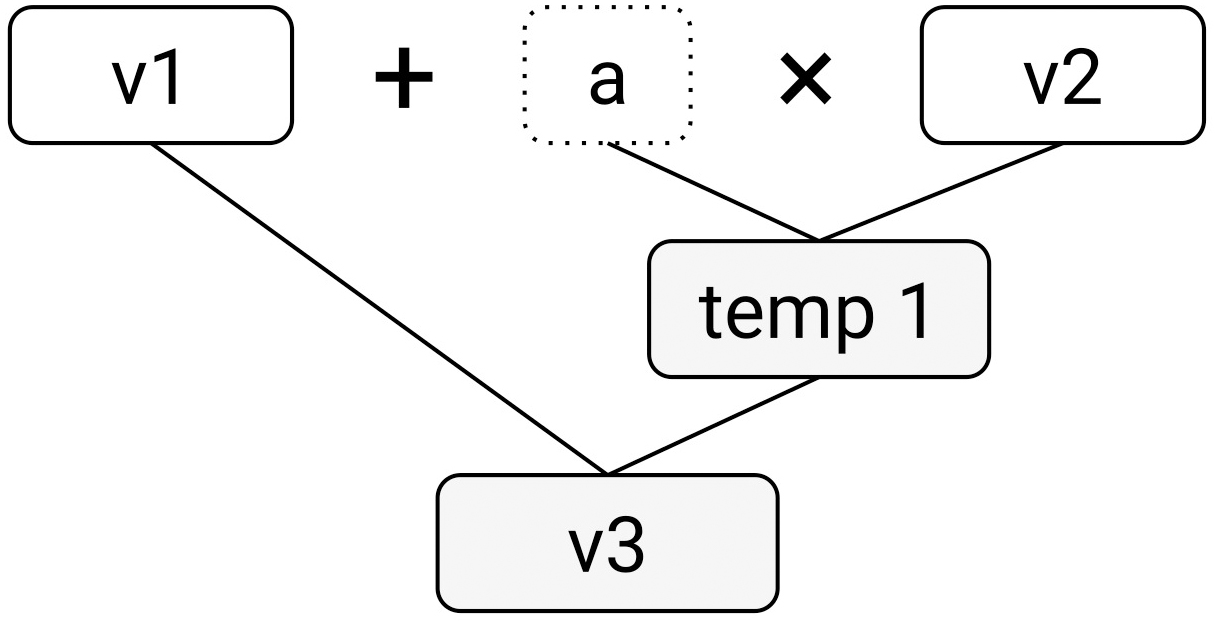
\includegraphics[width=0.5\textwidth]{content/3/chapter7/images/2.png}\\
图7.2:第一个表达式
\end{center}

下面显示的第二个图,给出了第二个表达式,v4 = v1 * v2 + v1 + v2计算的表示:

\begin{center}
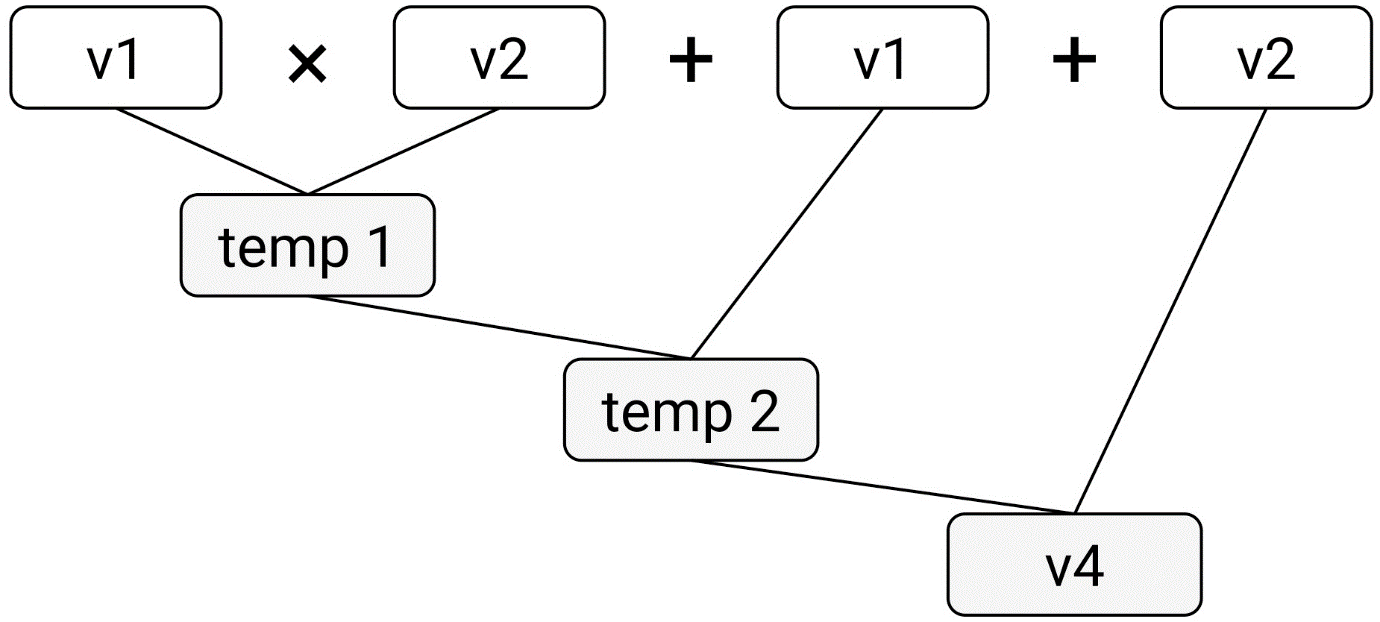
\includegraphics[width=0.5\textwidth]{content/3/chapter7/images/3.png}\\
图7.3:第二个表达式
\end{center}

为了避免这些临时变量,可以使用表达式模板模式重写vector类的实现:

\begin{itemize}
\item
定义类模板来表示两个对象之间的表达式(例如两个向量相加或相乘的表达式)。

\item
修改vector类并为其内部数据参数化容器,默认情况下,容器内部数据是std::vector,但也可以是表达式模板。

\item
更改重载的+和*操作符的实现。
\end{itemize}

从向量实现开始:

\begin{lstlisting}[style=styleCXX]
template<typename T, typename C = std::vector<T>>
struct vector
{
	vector() = default;
	
	vector(std::size_t const n) : data_(n) {}
	
	vector(std::initializer_list<T>&& l) : data_(l) {}
	
	
	vector(C const & other) : data_(other) {}
	template<typename U, typename X>
	vector(vector<U, X> const& other) : data_(other.size())
	{
		for (std::size_t i = 0; i < other.size(); ++i)
		data_[i] = static_cast<T>(other[i]);
	}

	template<typename U, typename X>
	vector& operator=(vector<U, X> const & other)
	{
		data_.resize(other.size());
		for (std::size_t i = 0; i < other.size(); ++i)
			data_[i] = static_cast<T>(other[i]);
		return *this;
	}

	std::size_t size() const noexcept
	{
		return data_.size();
	}
	
	T operator[](const std::size_t i) const
	{
		return data_[i];
	}

	T& operator[](const std::size_t i)
	{
		return data_[i];
	}

	C& data() noexcept { return data_; }
	
	C const & data() const noexcept { return data_; }
	
private:
	C data_;
};
\end{lstlisting}

除了初始实现中可用的操作外,还定义了以下操作:

\begin{itemize}
\item
默认构造函数

\item
容器的转换构造函数

\item
复制包含可能不同类型元素向量的复制构造函数

\item
来自包含可能不同类型元素向量的复制赋值操作符

\item
成员函数数据,提供对存储数据的底层容器的访问
\end{itemize}

表达式模板是一个简单的类模板,其存储两个操作数,并提供了一种执行操作求值的方法。本例中,需要实现两个向量相加、两个向量相乘,以及标量与向量相乘的表达式。来看看两个向量相加的表达式模板的实现:

\begin{lstlisting}[style=styleCXX]
template<typename L, typename R>
struct vector_add
{
	vector_add(L const & a, R const & b) : lhv(a), rhv(b) {}
	
	auto operator[](std::size_t const i) const
	{
		return lhv[i] + rhv[i];
	}

	std::size_t size() const noexcept
	{
		return lhv.size();
	}

private:
	L const & lhv;
	R const & rhv;
};
\end{lstlisting}

该类存储对两个向量的常量引用(或者,任何重载下标操作符,并提供size成员函数的类型)。表达式的求值发生在重载下标操作符中,而不是整个向量,只添加指定索引处的元素。

注意,此实现不处理不同大小的向量(可以将其作为练习进行更改)。但应该很容易理解这种方法的惰性性质,因为加法操作只在调用下标操作符时发生。

两个操作的乘法表达式模板,以类似的方式实现:

\begin{lstlisting}[style=styleCXX]
template<typename L, typename R>
struct vector_mul
{
	vector_mul(L const& a, R const& b) : lhv(a), rhv(b) {}
	
	auto operator[](std::size_t const i) const
	{
		return lhv[i] * rhv[i];
	}

	std::size_t size() const noexcept
	{
		return lhv.size();
	}

private:
	L const & lhv;
	R const & rhv;
};

template<typename S, typename R>
struct vector_scalar_mul
{
	vector_scalar_mul(S const& s, R const& b) :
		scalar(s), rhv(b)
	{}
	
	auto operator[](std::size_t const i) const
	{
		return scalar * rhv[i];
	}

	std::size_t size() const noexcept
	{
		return rhv.size();
	}

private:
	S const & scalar;
	R const & rhv;
};
\end{lstlisting}

更改的最后一部分是重载的+和*操作符的定义:

\begin{lstlisting}[style=styleCXX]
template<typename T, typename L, typename U, typename R>
auto operator+(vector<T, L> const & a,
vector<U, R> const & b)
{
	using result_type = decltype(std::declval<T>() +
								 std::declval<U>());
	return vector<result_type, vector_add<L, R>>(
		vector_add<L, R>(a.data(), b.data()));
}

template<typename T, typename L, typename U, typename R>
auto operator*(vector<T, L> const & a,
vector<U, R> const & b)
{
	using result_type = decltype(std::declval<T>() +
								 std::declval<U>());
	return vector<result_type, vector_mul<L, R>>(
		vector_mul<L, R>(a.data(), b.data()));
}

template<typename T, typename S, typename E>
auto operator*(S const& a, vector<T, E> const& v)
{
	using result_type = decltype(std::declval<T>() +
								 std::declval<S>());
	return vector<result_type, vector_scalar_mul<S, E>>(
		vector_scalar_mul<S, E>(a, v.data()));
}
\end{lstlisting}

尽管在实现此模式时代码更加复杂,但调用端代码不需要更改。这段代码没有任何修改,但以一种懒惰的方式实现。每个元素的求值,由vector类的复制构造函数和复制赋值操作符中的下标操作符触发。

若这个模式看起来很麻烦,那么还有更好的选择:范围库。

\subsubsubsection{7.6.1\hspace{0.2cm}使用范围库作为表达式模板的替代方案}

C++20的主要特性之一是范围库,其是容器的泛化——允许迭代其数据(元素)的类。范围库的一个关键元素是视图,是其他范围的非所有权包装器,通过某些操作转换底层范围。

此外,其是惰性求值的,构造、复制或销毁的时间不取决于底层范围的大小。惰性求值(即在元素被请求时应用转换,而不是在视图创建时)是该库的一个关键特性。然而,这正是表达式模板所支持的,所以表达式模板的许多用法可以用范围代替。

C++的范围库是基于Eric Niebler创建的range-v3库。这个库可以在\url{https://github.com/ericniebler/range-v3/}上获取。使用range-v3,可以编写以下代码来执行操作v1 + a * v2:

\begin{lstlisting}[style=styleCXX]
namespace rv = ranges::views;
std::vector<int> v1{ 1, 2, 3 };
std::vector<int> v2{ 4, 5, 6 };
double a { 1.5 };

auto sv2 = v2 |
		   rv::transform([&a](int val) {return a * val; });
auto v3 = rv::zip_with(std::plus<>{}, v1, sv2);
\end{lstlisting}

vector类不需要自定义实现,这只适用于std::vector容器,也不需要重载任何操作符。代码应该很容易理解,若对范围库比较熟悉的话。首先,创建一个视图,通过将每个元素与标量相乘来转换v2向量的元素。然后,创建第二个视图,将加号运算符应用于v1范围的元素和前一个操作生成的视图。

但这段代码不能使用标准库在C++20中编写,因为zip\_with视图没有包含在C++20中。但这个视图将在C++23中以zip\_view的名称提供。所以在C++23中,可以这样实现:

\begin{lstlisting}[style=styleCXX]
namespace rv = std::ranges::views;
std::vector<int> v1{ 1, 2, 3 };
std::vector<int> v2{ 4, 5, 6 };
double a { 1.5 };

auto sv2 = v2 |
           rv::transform([&a](int val) {return a * val; });
auto v3 = rv::zip_wiew(std::plus<>{}, v1, sv2);
\end{lstlisting}

为了结束对表达式模板模式的讨论,应该记住以下要点:该模式旨在为代价高昂的操作提供惰性求值,而这样做的代价是必须编写更多的代码(也可以说是更麻烦)和增加编译时间(因为沉重的模板代码将对此产生影响)。然而,从C++20开始,这个模式的替代可由范围库完成。

本章的下一节也是最后一节,我们将讨论类型列表。













